% !TEX root = ../prj4projektrapport.tex
% SKAL STÅ I TOPPEN AF ALLE FILER FOR AT MASTER-filen KOMPILERES 

\section{Funktionelle krav}

Funktionaliteten af systemet er beskrevet i 3 use cases, som beskriver brugerens interaktion med systemet. Den automatiske spændingsregulering er beskrevet særskilt i et diagram. Se dokumentation\footnote{Projektdokumentaion, 3.3, Funktionelle krav} for uddybning af efterfølgende krav. 

\subsubsection{Use case 1 - Start manuel mode}

\begin{figure}[H] % (alternativt [H])
	\centering
	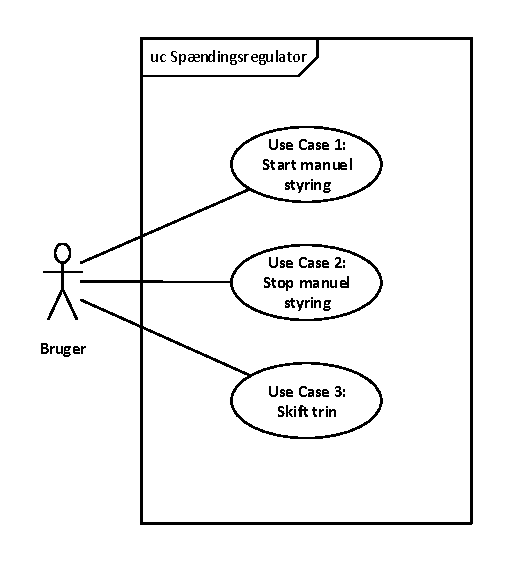
\includegraphics[width=0.5\textwidth]{Figure/UsecaseDiagram}
	\caption{Usecase Diagram}
	\label{fig:UsecaseDiagram}
\end{figure}